\documentclass[conference]{IEEEtran}
\IEEEoverridecommandlockouts

\usepackage{cite}
\usepackage{amsmath,amssymb}
\usepackage{fontspec}
\setmainfont{texgyretermes}[Extension=.otf,UprightFont=*-regular,BoldFont=*-bold,ItalicFont=*-italic,BoldItalicFont=*-bolditalic]
\usepackage{graphicx}
\usepackage{booktabs}
\usepackage{multirow}
\usepackage{array}
\usepackage{makecell}
\usepackage{xcolor}
\usepackage{algorithm}
\usepackage{algpseudocode}
\usepackage{tikz}
\usetikzlibrary{positioning,arrows.meta,fit}
\usepackage[hidelinks]{hyperref}

\newcommand{\pp}{\,pp}

\begin{document}

\title{PRISM: Predictive, Explainable System-Health Monitoring on a Personal Computer, with a Three-Model Comparison of Resource Forecasters}

\author{
\IEEEauthorblockN{Sahil Dhanuka}
\and
\IEEEauthorblockN{Shambhav Ghosh}
\and
\IEEEauthorblockN{Naresh Kumar Bishnoi}
}

\maketitle

\begin{abstract}
Desktop operating systems report resource usage only after a slowdown has
already happened. We present PRISM, a monitor for a personal computer that runs
entirely on the device. It forecasts CPU and memory utilisation 45\,s and
210\,s ahead, estimates the probability of resource contention, explains the
likely cause, and recommends an action. PRISM has 592 automated tests, a browser dashboard and a measured overhead
of 2.26\,\% CPU. To choose its
forecasting model, we compared three machine-learning regressors, LightGBM,
Random Forest and Ridge regression, on 113{,}876 samples (about 48\,h) of real
usage from one macOS machine. We first added a preprocessing stage fitted on
training data only. It removes rows whose history is incomplete after
collector gaps, log-transforms skewed byte rates, and drops constant and
near-duplicate features (254 to 224). All three models then used identical
inputs and chronological splits, under a selection rule fixed in advance.
LightGBM had the highest mean skill against a naive persistence forecast
($-0.113$, versus $-0.252$ for Random Forest and $-0.607$ for Ridge) and the
smallest worst-case loss (23\,\% versus 85\,\% and 179\,\%), and it was the
cheapest to run. It was therefore selected. The evidence is mixed, and we
report it as such. Preprocessing lifted Ridge's mean skill from $-0.98$ to
$-0.61$ and made it the best CPU forecaster; it is the only model that reliably
beats persistence (+12\,\% at 45\,s). Random Forest had the best
cross-validation record. A regime analysis explains the negative average
skill. On the 25\,\% of samples where CPU load actually changes, the learned
models cut error by 29--34\,\% against persistence. On the 75\,\% where
nothing changes, persistence is almost unbeatable, and those samples dominate
this idle-heavy machine. Expressed as accuracy (100\,\% minus mean absolute
error), LightGBM's forecasts are 97.9\,\% accurate on average, 96--97\,\% for
CPU and 99\,\% for memory.
\end{abstract}

\begin{IEEEkeywords}
system monitoring, time-series forecasting, LightGBM, random forest, ridge
regression, resource contention, explainable AI, walk-forward validation,
Diebold--Mariano test
\end{IEEEkeywords}

%=====================================================================
\section{Introduction}
%=====================================================================
Operating-system tools such as Activity Monitor on macOS and Task Manager on
Windows are \emph{reactive}. They show that the CPU is saturated or that
memory is swapping only after the user has already felt the slowdown. They
also report raw numbers, not causes. A user who sees ``memory pressure:
high'' still has to work out which process is responsible, whether the
pressure is growing, and what to do about it. Most users never open these
tools at all until the machine has already become unresponsive.

PRISM aims to make desktop monitoring \emph{predictive} and
\emph{explainable}. Every few seconds it answers four questions:
\begin{enumerate}
  \item Where will CPU and memory utilisation be in the next 30--60\,s
        (short horizon) and 2--5\,min (medium horizon)?
  \item How likely is resource contention in the short horizon?
  \item If contention is likely, what kind is it? Examples are a single
        runaway process, several competing processes, or gradual versus
        sudden memory pressure.
  \item What should the user do about it?
\end{enumerate}

Answering the first question well is the foundation for the others, because
the forecasts are inputs to the contention classifier and to the diagnosis.
The choice of forecasting model is therefore the most important modelling
decision in the system. We study it through three research questions.
\begin{description}
  \item[RQ1] Which of three standard ML regressors (boosted trees, bagged
        trees, a regularised linear model) forecasts desktop CPU and memory
        utilisation best on real usage data, and are the differences
        statistically significant?
  \item[RQ2] Why do the learned models struggle to beat a naive ``no
        change'' forecast, and where, if anywhere, do they add value?
  \item[RQ3] Which features does the chosen model actually rely on?
\end{description}

This paper makes four contributions:
\begin{itemize}
  \item \textbf{A complete on-device pipeline}, from threaded metric
        collection to a browser dashboard. The same
        feature-engineering code is used for training and live inference.
        The pipeline has an explicit deployment gate and human-confirmed
        retraining (Section~\ref{sec:system}).
  \item \textbf{A leakage-free preprocessing stage and a controlled
        comparison of three ML forecasters} on real usage data, run with and
        without preprocessing, with a selection rule fixed in advance
        (Sections~\ref{sec:setup} and \ref{sec:results}).
  \item \textbf{A statistical and diagnostic analysis} that goes beyond
        average error. It includes Diebold--Mariano tests, block-bootstrap
        confidence intervals, a stable-versus-moving regime analysis and
        feature attribution.
  \item \textbf{An honest account of the limits} of the result, and of how
        the system's own gate stops a weak model from being deployed
        (Section~\ref{sec:discussion}).
\end{itemize}

%=====================================================================
\section{Related Work}
%=====================================================================
\subsection{Workload and resource forecasting}
Most resource prediction work targets servers and clouds, where forecasts
drive autoscaling. PRESS~\cite{gong2010press} used signal processing and
Markov chains to predict resource demand for elastic scaling.
Roy \emph{et al.}~\cite{roy2011autoscaling} and Calheiros
\emph{et al.}~\cite{calheiros2015arima} used ARIMA-family models for workload
forecasting and measured their effect on quality of service. These systems
see aggregated, fairly smooth demand from many users. PRISM differs in two
ways. First, it targets a single interactive personal computer, where load is
dominated by long idle periods broken by short, user-driven bursts. Second, it
runs both training and inference on that same machine under a strict overhead
budget, so model cost is a first-class concern. Table~\ref{tab:related}
summarises the differences, including from the built-in tools PRISM aims to
improve on.

\begin{table}[t]
\centering
\caption{PRISM compared with existing tools and work}
\label{tab:related}
\footnotesize\setlength{\tabcolsep}{3pt}
\begin{tabular}{@{}p{2.2cm}cccc@{}}
\toprule
& \makecell{Activity\\Monitor /\\Task Mgr.} & \makecell{PRESS\\\cite{gong2010press}} & \makecell{ARIMA\\\cite{roy2011autoscaling,calheiros2015arima}} & \makecell{\textbf{PRISM}} \\
\midrule
Target        & PC & cloud & cloud & \textbf{PC} \\
Predicts load & no & yes & yes & \textbf{yes} \\
Method        & -- & FFT + Markov & ARIMA & \textbf{LightGBM} \\
Explains cause & no & no & no & \textbf{SHAP} \\
Advises user  & no & auto-scales & auto-scales & \textbf{3 actions} \\
Flags anomalies & no & no & no & \textbf{Isol.\ Forest} \\
Trains on device & -- & no & no & \textbf{yes, gated} \\
\bottomrule
\end{tabular}
\end{table}

\subsection{Model families for tabular forecasting}
Gradient boosting~\cite{friedman2001gbm} builds an additive model of shallow
trees, each fitted to the residuals of the ensemble so far.
XGBoost~\cite{chen2016xgboost} and LightGBM~\cite{ke2017lightgbm} made the
approach fast and scalable. LightGBM uses histogram-based split finding and
grows trees leaf-wise. Random Forests~\cite{breiman2001rf} instead average many
deep, decorrelated trees, which reduces variance. Ridge
regression~\cite{hoerl1970ridge} is the standard regularised linear baseline.
On medium-sized tabular data, tree ensembles remain very hard to beat, even for
deep networks~\cite{grinsztajn2022tree}. We therefore compare the two main
tree-ensemble families against a linear model rather than against deep
sequence models, which would also be too expensive to retrain on the user's
own machine.

\subsection{Anomaly detection and explainability}
Anomaly detection is a broad field~\cite{chandola2009anomaly}. Isolation
Forest~\cite{liu2008iforest} is popular for unsupervised scoring because it is
fast and needs no labels. SHAP~\cite{lundberg2017shap} gives consistent
per-prediction feature attributions, and TreeSHAP~\cite{lundberg2020treeshap}
computes them exactly and quickly for tree ensembles. This is one practical
reason to prefer a tree model when predictions must be explained to a user.

\subsection{Evaluating forecasts}
Random $k$-fold cross-validation leaks future information into training for
time series. Rolling-origin (walk-forward) evaluation is the accepted
alternative~\cite{tashman2000,bergmeir2012}. Scale-free comparison against a
naive forecast~\cite{hyndman2006accuracy,hyndman2021fpp} is the usual way to
judge whether a model has any real skill. Whether one forecaster is
significantly more accurate than another is tested with the Diebold--Mariano
(DM) test~\cite{diebold1995dm}, using a variance estimate that is robust to
autocorrelation~\cite{newey1987hac}. For confidence intervals on dependent
data, the moving-block bootstrap~\cite{kunsch1989block} resamples contiguous
blocks, not individual points. We use all of these.

%=====================================================================
\section{Problem Formulation}\label{sec:problem}
%=====================================================================
Let $\mathbf{m}_t$ be the vector of system metrics sampled at time $t$. These
are CPU\,\%, memory\,\%, swap\,\%, one-minute load average, and disk and
network byte rates. Let $\mathbf{p}_t$ be a summary of the process table at
$t$. A feature map $\phi$ turns the recent history into a fixed-length vector
$\mathbf{x}_t=\phi(\mathbf{m}_{\le t},\mathbf{p}_{\le t})\in\mathbb{R}^{254}$,
using only data at or before $t$.

\subsection{Forecasting}
For a metric $y\in\{\text{CPU\,\%},\text{memory\,\%}\}$ and a horizon
$h\in\{45\,\text{s},210\,\text{s}\}$ (the midpoints of the two horizon
ranges), we learn a function $f$ that predicts the \emph{change}, not the
level:
\begin{equation}
  \hat y_{t+h} = y_t + f(\mathbf{x}_t), \qquad
  f = \arg\min_{f} \sum_t \ell\big(y_{t+h}-y_t,\; f(\mathbf{x}_t)\big).
\end{equation}
Predicting the delta makes ``no change'' the natural zero of the model. It
also removes the slowly varying level, which a tree model cannot extrapolate
beyond its training range. Four such models are trained: two metrics times
two horizons.

\subsection{Contention}
A sample is labelled as contention if any tracked metric $k$ reaches its
threshold $\tau_k$ at the short horizon:
\begin{equation}
  c_t = \mathbb{1}\Big[\max_k \big(m_{k,t+h_s} - \tau_k\big) \ge 0\Big].
\end{equation}
The thresholds are CPU 70\,\%, memory 85\,\%, swap 50\,\% and 50\,kB/s for
each disk and network byte rate. A classifier estimates $P(c_t=1\mid\mathbf{x}_t)$.

\subsection{Evaluation measures}
For $n$ holdout samples with error $e_t=y_{t+h}-\hat y_{t+h}$, we report
$\mathrm{MAE}=\frac1n\sum|e_t|$ and $\mathrm{RMSE}=\sqrt{\frac1n\sum e_t^2}$
in percentage points (pp). \emph{Directional accuracy} is the fraction of
samples where the predicted direction (rising, falling or stable) matches the
actual one. A change within 2\,\% of the current value (relative) counts as
stable. The primary measure is \emph{skill} against the naive persistence
forecast $\hat y_{t+h}=y_t$:
\begin{equation}
  S = 1 - \frac{\mathrm{MAE}_{\text{model}}}{\mathrm{MAE}_{\text{persistence}}}.
  \label{eq:skill}
\end{equation}
$S>0$ means the model beats ``no change'', $S=0$ means it ties, and $S<0$
means it is worse. For example, $S=-0.18$ means 18\,\% more error than
persistence.

%=====================================================================
\section{System Design}\label{sec:system}
%=====================================================================

\begin{figure}[t]
\centering
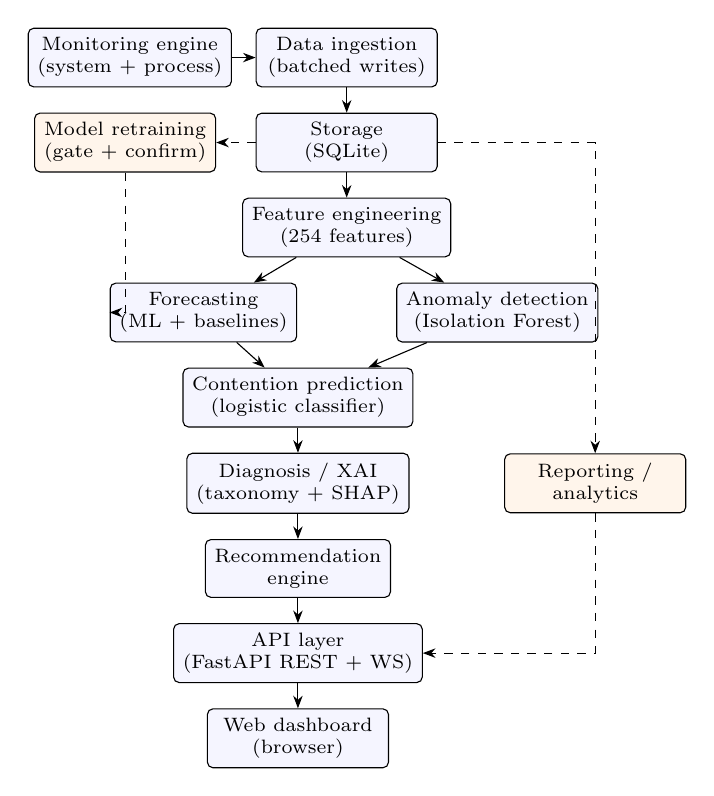
\begin{tikzpicture}[
  node distance=3.2mm and 3mm,
  box/.style={draw, rounded corners=2pt, align=center, font=\scriptsize,
              minimum width=23mm, minimum height=6mm, fill=blue!4},
  side/.style={box, fill=orange!8},
  arr/.style={-{Stealth[length=1.6mm]}, thin},
  dsh/.style={arr, dashed}]
\node[box] (mon) {Monitoring engine\\(system + process)};
\node[box, right=of mon] (ing) {Data ingestion\\(batched writes)};
\node[box, below=of ing] (sto) {Storage\\(SQLite)};
\node[box, below=of sto] (feat) {Feature engineering\\(254 features)};
\node[box, below left=of feat, xshift=10mm] (fc) {Forecasting\\(ML + baselines)};
\node[box, below right=of feat, xshift=-10mm] (an) {Anomaly detection\\(Isolation Forest)};
\node[box, below=of fc, xshift=12mm] (ct) {Contention prediction\\(logistic classifier)};
\node[box, below=of ct] (dg) {Diagnosis / XAI\\(taxonomy + SHAP)};
\node[box, below=of dg] (rc) {Recommendation\\engine};
\node[box, below=of rc] (api) {API layer\\(FastAPI REST + WS)};
\node[box, below=of api] (ui) {Web dashboard\\(browser)};
\node[side, left=of sto, xshift=-2mm] (rt) {Model retraining\\(gate + confirm)};
\node[side, right=of dg, xshift=9mm] (rep) {Reporting /\\analytics};
\draw[arr] (mon) -- (ing); \draw[arr] (ing) -- (sto); \draw[arr] (sto) -- (feat);
\draw[arr] (feat) -- (fc); \draw[arr] (feat) -- (an);
\draw[arr] (fc) -- (ct); \draw[arr] (an) -- (ct);
\draw[arr] (ct) -- (dg); \draw[arr] (dg) -- (rc); \draw[arr] (rc) -- (api);
\draw[arr] (api) -- (ui);
\draw[dsh] (sto) -- (rt); \draw[dsh] (rt) |- (fc);
\draw[dsh] (sto.east) -| (rep); \draw[dsh] (rep) |- (api);
\end{tikzpicture}
\caption{PRISM's pipeline. Solid arrows show the live inference
cycle, which runs every 5\,s. Dashed arrows show loops that run on their own
cadence: retraining on accumulated real usage, and reporting.}
\label{fig:arch}
\end{figure}

Fig.~\ref{fig:arch} shows the pipeline. It is implemented in Python~3.12. The
main libraries are \texttt{psutil}~7.2 for metrics, SQLAlchemy~2.0 over
SQLite, LightGBM~4.7, scikit-learn~1.9, statsmodels~0.14, SHAP~0.52 and
FastAPI~0.141. The dashboard is plain JavaScript with uPlot charts and needs no
build step.

\subsection{Data collection and storage}
Background threads poll system metrics every 1.5\,s. They poll the process
table every 3\,s, storing the top 20 processes by CPU and the top 20 by memory
individually and aggregating the rest into one row. A typical desktop has
around 180 processes, so this cuts storage by an order of magnitude. A bounded
queue of 20{,}000 items feeds batched, ordered writes of 200 rows or every
5\,s, whichever comes first. Retention is 72\,h at full resolution for system
metrics, after which rows are rolled up, and 6\,h for raw process rows.
Durable per-poll process summaries are computed and stored \emph{before} the
raw rows are pruned, so multi-day training data keeps its process signal.

\subsection{Feature engineering}
One pure function builds the feature matrix for both training and live
inference. This removes train/serve skew by construction, and a dedicated test
checks that a live feature vector equals the training vector for the same
timestamp. A second test checks causality: no feature uses data from after
$t$. Table~\ref{tab:features} summarises the 254 features. A separate
preprocessing stage (Section~\ref{sec:preprocessing}) then cleans the
feature matrix before any model sees it.

\begin{table}[t]
\centering
\caption{Feature groups (254 columns in total)}
\label{tab:features}
\begin{tabular}{@{}p{2.1cm}rp{4.6cm}@{}}
\toprule
Group & Cols & Examples \\
\midrule
Current value  & 1   & metric value at $t$ \\
Lagged values  & 16  & value 1--$k$ samples ago \\
Rate of change & 8   & per-second slope of each gauge \\
Rolling-window & 64  & mean, std, min, max over 30\,s and 120\,s \\
Process activity & 165 & launches in 30/120\,s, terminations in 30\,s, launch bursts in 10\,s, activity of processes younger than 60\,s, top-1/top-5 CPU and RSS shares, thread counts (and their rolling statistics) \\
\bottomrule
\end{tabular}
\end{table}

\subsection{Live inference loop}
Algorithm~\ref{alg:loop} shows one inference cycle, which runs every 5\,s.
This is deliberately slower than the 1.5\,s polling rate, because each cycle
(especially a SHAP explanation) costs more than one poll, and the 3\,\% CPU
budget covers inference as well as collection.

\begin{algorithm}[t]
\caption{One live-inference cycle (every 5\,s)}
\label{alg:loop}
\begin{algorithmic}[1]
\State $\mathbf{x}_t \gets \phi(\text{recent metrics and process summaries})$
\For{each metric $y$ and horizon $h$}
  \State $\hat y_{t+h} \gets y_t + f_{y,h}(\mathbf{x}_t)$ \Comment{active model}
  \State $c_{y,h} \gets \mathrm{clip}(1-\mathrm{RMSE}_{\text{val}}/\sigma_y,\,0,\,1)$
\EndFor
\State $a_t \gets$ IsolationForest score of $\mathbf{x}_t$ in $[0,1]$
\State $p_t \gets P(c_t{=}1\mid\mathbf{x}_t,\hat{\mathbf{y}})\cdot(1-0.3\,a_t)$
\If{$p_t \ge \tau$}
  \State category $\gets$ \Call{Diagnose}{SHAP top-5, top processes}
  \State actions $\gets$ \Call{Catalog}{category}
\EndIf
\State store all outputs; push state to WebSocket clients
\end{algorithmic}
\end{algorithm}

The confidence $c_{y,h}$ in line~4 is a single number between 0 and 1. It
is 1 for a perfect validation fit and 0 when the validation RMSE is as large as
the target's own standard deviation. It is not a calibrated interval. Line~7
\emph{damps} the contention probability when the current state looks
anomalous. The classifier was trained on normal patterns, so its output is
less trustworthy on unusual inputs. The decision threshold $\tau$ is fitted
on held-out data as the point of the precision--recall curve with the highest
F1 score; for the deployed classifier it is 0.50. When the held-out labels
contain only one class, the curve is unusable and $\tau$ falls back to 0.75,
which favours precision over recall: a false alarm costs user trust, while a
missed alarm costs only a warning that the user would not have had anyway.

\subsection{Diagnosis and recommendation}
When contention is predicted, the top five attributed features are mapped to
coarse resource types (CPU, memory, disk, network). If no type accounts for at
least 60\,\% of the total attribution, the event is \emph{cross-resource}
contention. Otherwise the dominant type chooses the category, refined by
further rules. Table~\ref{tab:taxonomy} lists the eight categories. Each
actionable category maps to three curated actions (21 in total) from a
versioned catalogue. The anomaly category is deliberately not actionable,
because recommending an action for a pattern the system does not understand
would be guesswork. Every diagnosis has a technical explanation and a
plain-language one.

\begin{table}[t]
\centering
\caption{Diagnosis taxonomy and an example recommended action}
\label{tab:taxonomy}
\begin{tabular}{@{}p{2.7cm}p{2.3cm}p{2.4cm}@{}}
\toprule
Category & Rule & Example action \\
\midrule
CPU, single process & top process $\ge$50\,\% of top-5 CPU & Quit or pause the dominant process \\
CPU, multi-process & CPU dominant, no single leader & Stagger simultaneous heavy tasks \\
Memory, gradual & mem.\ rate $<$0.2\pp/s & Close unused tabs and idle apps \\
Memory, sudden & mem.\ rate $\ge$0.2\pp/s & Identify what just launched \\
Disk I/O bottleneck & disk dominant & Let the current disk job finish \\
Network saturation & network dominant & Pause large downloads \\
Cross-resource & no type $\ge$60\,\% & Reduce concurrent workload \\
Unusual pattern & anomaly score high & (none: not actionable) \\
\bottomrule
\end{tabular}
\end{table}

\subsection{Deployment gate and retraining}\label{sec:gate}
Three statistical baselines are always trained alongside the ML forecaster:
persistence, a moving average and Holt exponential smoothing. An ML forecaster
is deployed only if its mean walk-forward MAE beats the \emph{best} of them by
at least 5\,\% (relative). Otherwise the best baseline serves predictions. A
retraining candidate must also beat persistence by 5\,\% on the chronological
holdout and exceed 55\,\% directional accuracy. The gate's decision and its
evidence are always stored. Retraining never deploys automatically: an
operator must confirm through the CLI, the API or the dashboard's Model view, and any
deployment can be rolled back. This rule is why a weak model cannot silently
reach the live dashboard.

\subsection{API and user interface}
A FastAPI server exposes 28 REST routes (health, readiness, live state,
history, reporting, model comparison, retraining, confirm and rollback) and one
WebSocket, \texttt{/ws/live}, that pushes each cycle's state. The same server
serves a browser dashboard with five views. \emph{Live}
(Fig.~\ref{fig:dashboard}) shows current usage and contention risk, live
charts of actual versus forecast values with a confidence band, the contention
probability against its threshold, the diagnosis in plain language, the
recommended actions and the top contributing processes. \emph{Accuracy} plots
predicted against actual values over a chosen window. \emph{Reports} gives a
daily or weekly summary. \emph{Compare} draws the saved results of the model
comparison in Section~\ref{sec:results} on demand: accuracy, error, error
relative to persistence and directional accuracy per target, the
stable-versus-moving split, the cross-validation folds and running cost.
\emph{Model} shows the active version and is where an operator confirms or
rolls back a retrained model. An earlier PySide6 desktop client is still
included but is no longer the main interface. A record/replay tool plays back a real recorded
pressure event into a separate database at any speed, for reproducible
demonstrations.

\begin{figure}[t]
\centering
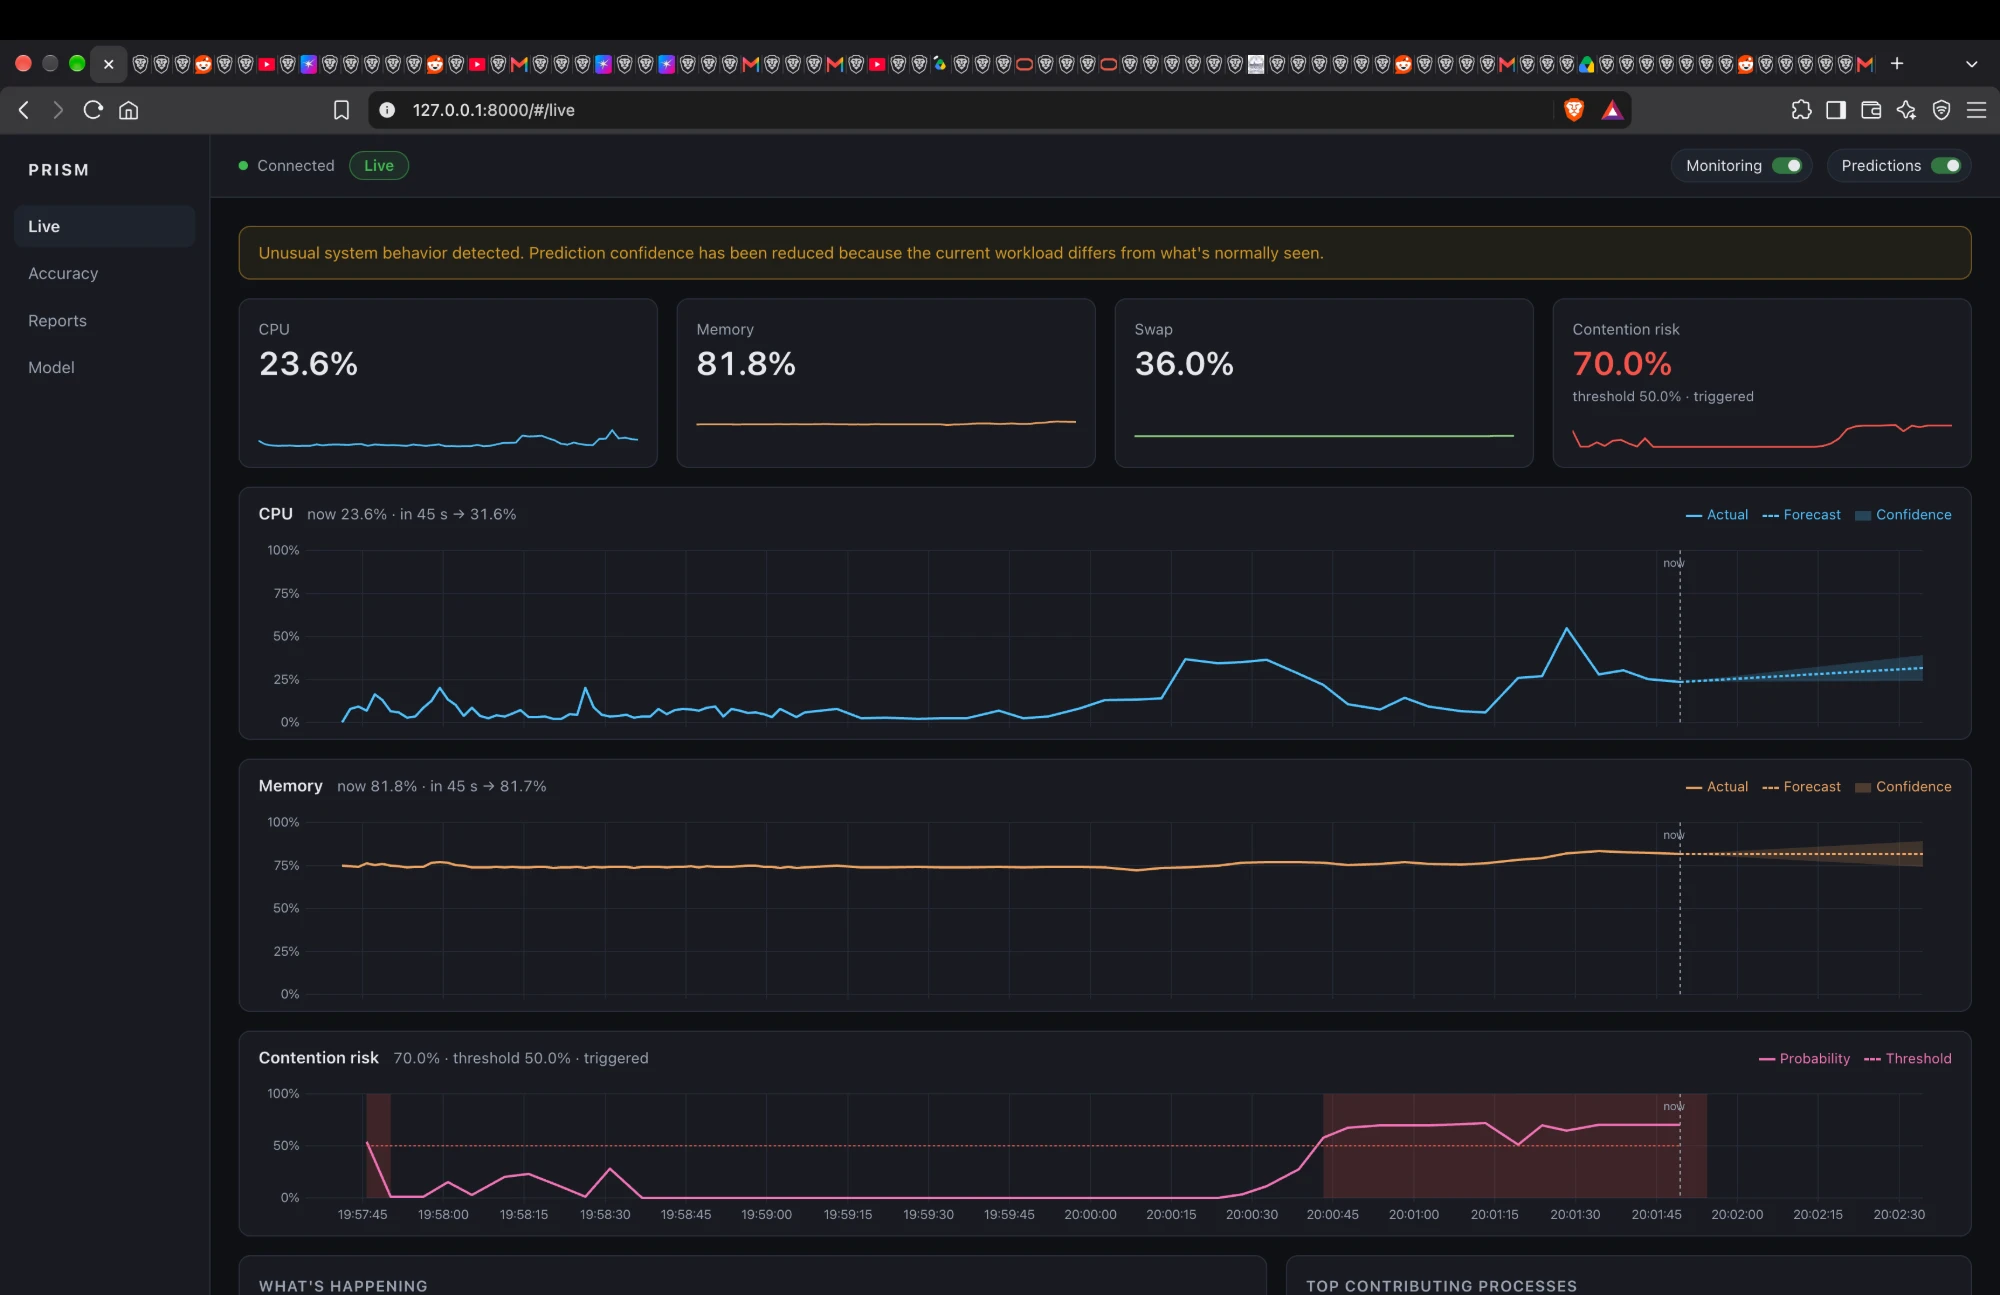
\includegraphics[width=\columnwidth]{figures/live_dashboard_web.png}
\caption{The dashboard's Live view during a real memory-pressure event on the
test machine. Contention risk has risen to 70\,\% against the fitted 50\,\%
threshold, and the anomaly detector has flagged the workload as unusual, so
prediction confidence is reduced. Below the charts (not shown) the diagnosis
reads ``Memory usage is climbing steadily'' and the first recommended action
is to close unused browser tabs. After the tabs were closed, memory fell from
82\,\% to 63\,\% and the risk returned to 0\,\%.}
\label{fig:dashboard}
\end{figure}

\subsection{Engineering quality}
The system has 592 automated tests: 568 Python tests (Table~\ref{tab:modules})
and 24 JavaScript unit tests for the dashboard's numeric helpers. Each Python test is
tagged either \emph{behavioural}, meaning it asserts that a computed value is
correct, or \emph{plumbing}, meaning it only asserts that code ran. The tag is
enforced by the test runner, so a large test count cannot hide a module that
is never checked for correctness. Every module has at least one behavioural
test. Monitoring overhead was measured in isolation at 2.26\,\% CPU against a
3\,\% budget, and database growth at 3.48\,MB/h against a 200\,MB/h ceiling.

\begin{table}[t]
\centering
\caption{Python tests per module (B = behavioural, P = plumbing). The
dashboard's 24 JavaScript tests run separately under Node.}
\label{tab:modules}
\begin{tabular}{@{}lrrr@{}}
\toprule
Module & Tests & B & P \\
\midrule
Data storage & 31 & 14 & 17 \\
Monitoring + ingestion & 35 & 17 & 18 \\
Feature engineering & 45 & 29 & 16 \\
Preprocessing & 9 & 8 & 1 \\
Forecasting & 54 & 39 & 15 \\
Contention + anomaly & 76 & 48 & 28 \\
Diagnosis / XAI & 40 & 40 & 0 \\
Recommendation & 14 & 7 & 7 \\
Model lifecycle (gate, deploy) & 37 & 27 & 10 \\
Model comparison + evaluation & 8 & 3 & 5 \\
API layer & 63 & 16 & 47 \\
Reporting / analytics & 26 & 23 & 3 \\
Web dashboard & 6 & 2 & 4 \\
Desktop client (legacy) & 54 & 28 & 26 \\
Cross-cutting (CLI, config, replay, \dots) & 70 & 40 & 30 \\
\midrule
\textbf{Total} & \textbf{568} & \textbf{341} & \textbf{227} \\
\bottomrule
\end{tabular}
\end{table}

%=====================================================================
\section{Experimental Setup}\label{sec:setup}
%=====================================================================

\subsection{Data}
The data is real, passively collected usage of one macOS development machine
between 17 and 23~September~2026. The machine was used normally and no load was
generated artificially. The wall-clock window is 130\,h. The collector was off
for two long stretches (41.0\,h and 12.2\,h) and paused 140 more times for
periods of 30\,s to a few minutes, mostly when the laptop slept. The data covers
about 47.7\,h of recorded time (113{,}876 samples at 1.5\,s). The split is
chronological with no shuffling. The oldest 80\,\% of samples (91{,}100) are
used for training and the newest 20\,\% (22{,}776, from 20~September
10:07~UTC) are held out. To keep every number in this paper reproducible, all
analyses run on a frozen copy of the database trimmed to this window.

\begin{figure}[t]
\centering
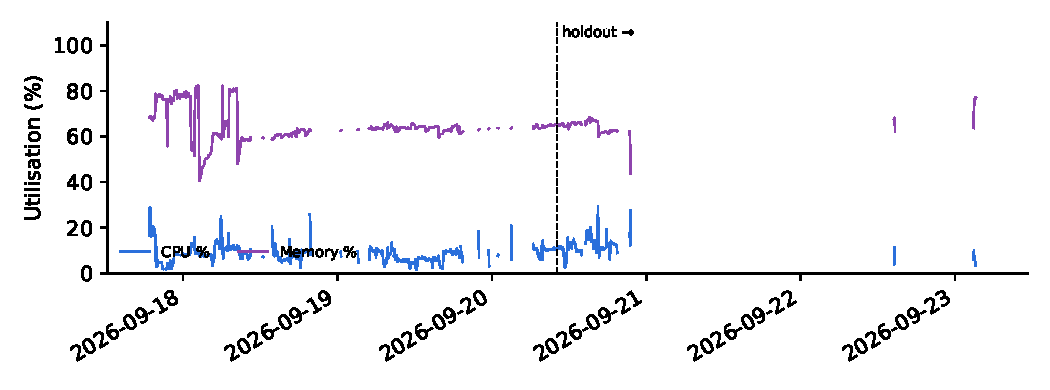
\includegraphics[width=\columnwidth]{figures/timeseries.pdf}
\caption{CPU and memory utilisation over the collection window (5-min means).
Blank stretches are periods when the collector was off. The dashed line marks
the start of the holdout.}
\label{fig:timeseries}
\end{figure}

\begin{figure}[t]
\centering
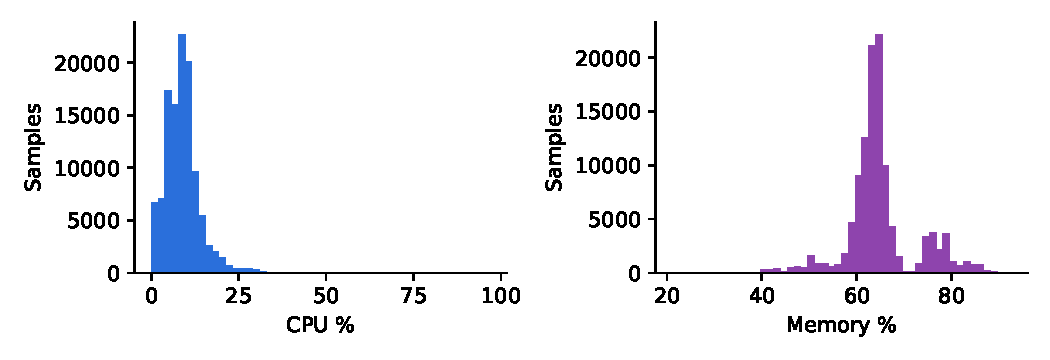
\includegraphics[width=\columnwidth]{figures/distributions.pdf}
\caption{Distribution of CPU and memory utilisation across all 113{,}876
samples. CPU is below 20\,\% in 96.7\,\% of samples.}
\label{fig:dist}
\end{figure}

Figs.~\ref{fig:timeseries} and \ref{fig:dist} characterise the data, which is
strongly idle-dominated. Median CPU is 8.8\,\%, the 90th percentile is
14.4\,\% and the 99th is 27.7\,\%. CPU is below 10\,\% in 65.0\,\% of samples
and below 20\,\% in 96.7\,\%. It reaches the 70\,\% contention threshold in
only nine samples (0.008\,\%). Memory is more stable still: the median is
64.0\,\%, 80\,\% of samples lie between 59.0 and 76.5\,\%, and 1.2\,\% are at
or above 85\,\%. On a machine that is mostly idle, the best estimate of the
next value is usually the current value, and this shapes every result below.

\subsection{Data preprocessing}\label{sec:preprocessing}
Feature engineering already performs the per-sample cleaning that any row
needs: it sorts and de-duplicates timestamps, turns cumulative counters into
per-second rates, treats a counter reset or a gap above 30\,s as missing, and
leaves a lag feature blank rather than reaching across a gap. We audited the
raw data before modelling. It contains no duplicate timestamps, no
out-of-order samples, no infinite values and no percentages outside
0--100\,\%. It does contain four problems that per-sample cleaning cannot fix,
because they depend on the dataset as a whole:
\begin{itemize}
  \item \emph{Incomplete history after gaps.} A ``120\,s rolling mean''
        computed 3\,s after the collector restarts is really a mean of two
        samples.
  \item \emph{Near-duplicate features.} 29 feature pairs are correlated
        above 0.99, for example a lag and a rolling minimum of the same
        slowly changing process count.
  \item \emph{A constant feature.} One process statistic never varies in the
        training data.
  \item \emph{Heavy skew.} Disk and network byte rates reach skewness of 65:
        a download is orders of magnitude above idle traffic.
\end{itemize}

We therefore added a preprocessing stage between feature engineering and the
models (Table~\ref{tab:prep}). It is implemented as a tested module of the
system (\texttt{features/preprocessing.py}, 9 tests). It has two kinds of
step. \emph{Row} steps are stateless and applied to training and test rows
alike. \emph{Column} steps are \emph{fitted}: which columns to transform or
drop is decided from training rows only, then applied unchanged to validation
and test rows. In walk-forward cross-validation the column steps are refitted
inside every fold, so no information from any evaluation slice leaks into the
choice. Missing values are deliberately left as blanks for the tree models,
which split on them natively. Ridge fills them with the training median and
standardises every feature inside its own pipeline, again fitted on training
rows only.

\begin{table}[t]
\centering
\caption{Preprocessing steps and their effect (45\,s targets; 210\,s in
parentheses where different)}
\label{tab:prep}
\footnotesize\setlength{\tabcolsep}{3pt}
\begin{tabular}{@{}p{1.9cm}p{3.3cm}>{\raggedright\arraybackslash}p{2.6cm}@{}}
\toprule
Step & Rule & Effect \\
\midrule
\multicolumn{3}{@{}l}{\emph{Rows (stateless)}} \\
1. Validity & drop non-finite values or values outside 0--100\,\% & 0 rows \\
2. Warm-up & drop the first 120\,s after each gap $>$30\,s & 581 (578) train, 407 (320) test \\
\multicolumn{3}{@{}l}{\emph{Columns (fitted on training rows)}} \\
3. Log transform & $\mathrm{sign}(x)\log(1+|x|)$ on byte-rate features & 44 columns \\
4. Constant & drop zero-variance columns & 1 column \\
5. Redundant & drop the later of any pair with $|r|>0.99$ & 29 columns \\
\midrule
\multicolumn{2}{@{}l}{Result} & 254\,$\to$\,224 features \\
& & 90{,}313\,$\to$\,89{,}732 train rows \\
& & 22{,}557\,$\to$\,22{,}150 test rows \\
\bottomrule
\end{tabular}
\end{table}

The row counts in Table~\ref{tab:prep} are slightly below the raw sample
counts. The supervised dataset already excludes samples that have no measured
value exactly one horizon later, which happens just before every gap. Many of
the 140 short gaps are brief wake-ups from sleep, with only a few samples
between two pauses. Those samples have no future value, so the pauses around
them merge. The training timeline therefore splits into 14 contiguous segments
at the 45\,s horizon and 19 at 210\,s, and warm-up rows are removed at the
start of each.

\subsection{Candidates}
Table~\ref{tab:cands} lists the three candidates. LightGBM uses PRISM's
production hyperparameters unchanged. The other two use common, sensible
settings, implemented with scikit-learn~\cite{pedregosa2011sklearn}. No
candidate was tuned on the test data. All three receive exactly the same
preprocessed feature matrix and the same delta target.

\begin{table}[t]
\centering
\caption{Candidate models and configuration}
\label{tab:cands}
\begin{tabular}{@{}p{1.7cm}p{2.4cm}p{3.2cm}@{}}
\toprule
Model & Family & Configuration \\
\midrule
LightGBM~\cite{ke2017lightgbm} & Gradient-boosted trees & 80 rounds, 15 leaves, learning rate 0.1, $\ge$5 samples/leaf; NaN handled natively \\
Random Forest~\cite{breiman2001rf} & Bagged trees & 100 trees, max depth 12, $\ge$5 samples/leaf, seed 0 \\
Ridge~\cite{hoerl1970ridge} & Regularised linear & $\alpha=1$; median imputation and standardisation \\
\midrule
\textit{Persistence} & \textit{Reference} & $\hat y_{t+h}=y_t$ (not a candidate) \\
\bottomrule
\end{tabular}
\end{table}

\subsection{Protocol}
Each candidate is first evaluated with 4-fold walk-forward cross-validation
(expanding window) on the training portion~\cite{tashman2000,bergmeir2012}. In
fold $k$, it trains on the first $k$ blocks and is scored on block $k{+}1$.
The preprocessing column steps are refitted on each fold's training blocks. The
candidate is then refitted on all training rows and scored once on the
untouched test rows. We record MAE, RMSE, directional accuracy, fit time,
median single-row prediction latency (over 200 predictions) and serialised
model size. Fit time and latency include the preprocessing step, because the
live system would have to pay for it too.

\subsection{Selection rule}
The rule was written into the comparison script before its first run, so the
choice could not be fitted to the numbers. The winner is the candidate with
the highest mean holdout skill (Eq.~\ref{eq:skill}) across the four targets.
If two candidates are within 0.02 of each other, the one with lower
prediction latency wins, because the forecaster runs every cycle.

\subsection{Statistical analysis}
Mean errors alone cannot tell whether a difference is real. We therefore use
three further tools.
\begin{itemize}
  \item \textbf{Diebold--Mariano test}~\cite{diebold1995dm}. It tests the
        per-sample loss difference $d_t=|e^{A}_t|-|e^{B}_t|$, with a
        Newey--West variance~\cite{newey1987hac} whose lag equals the horizon
        in samples (30 for 45\,s, 140 for 210\,s). Consecutive errors
        overlap and are strongly autocorrelated, so an ordinary $t$-test
        would overstate significance.
  \item \textbf{Moving-block bootstrap}~\cite{kunsch1989block}. It gives
        95\,\% confidence intervals for each skill score, using 1{,}000
        resamples of 400-sample (10-minute) blocks.
  \item \textbf{Regime split}. Test rows are divided by the size of the
        actual change $|y_{t+h}-y_t|$. The \emph{stable} regime is the
        smallest 75\,\% and the \emph{moving} regime is the largest
        25\,\%. The cut-offs are 3.8\pp{} and 5.0\pp{} for CPU at 45\,s and
        210\,s, and 0.6\pp{} and 0.9\pp{} for memory. This split uses the
        realised outcome, so it is a \emph{diagnostic} tool that shows where
        each model gains or loses. It is not a deployable rule.
\end{itemize}

%=====================================================================
\section{Results}\label{sec:results}
%=====================================================================
All results in this section use the preprocessed data unless stated
otherwise. Section~\ref{sec:prepeffect} compares them with the same
experiment run on raw features.

\subsection{Holdout accuracy (RQ1)}

\begin{table}[t]
\centering
\caption{Holdout MAE in percentage points (22{,}150 test rows at 45\,s,
21{,}733 at 210\,s). Lower is better; \textbf{bold} marks the best of the
three candidates.}
\label{tab:holdout}
\begin{tabular}{@{}lcccc@{}}
\toprule
Target & LightGBM & Rand.\ Forest & Ridge & \textit{Persist.} \\
\midrule
CPU, 45\,s   & 2.954 & 3.126 & \textbf{2.662} & \textit{3.017} \\
CPU, 210\,s  & 3.702 & \textbf{3.339} & 3.365 & \textit{3.550} \\
Mem, 45\,s   & 0.643 & \textbf{0.632} & 0.970 & \textit{0.536} \\
Mem, 210\,s  & \textbf{0.942} & 1.415 & 2.131 & \textit{0.765} \\
\bottomrule
\end{tabular}
\end{table}

\begin{figure}[t]
\centering
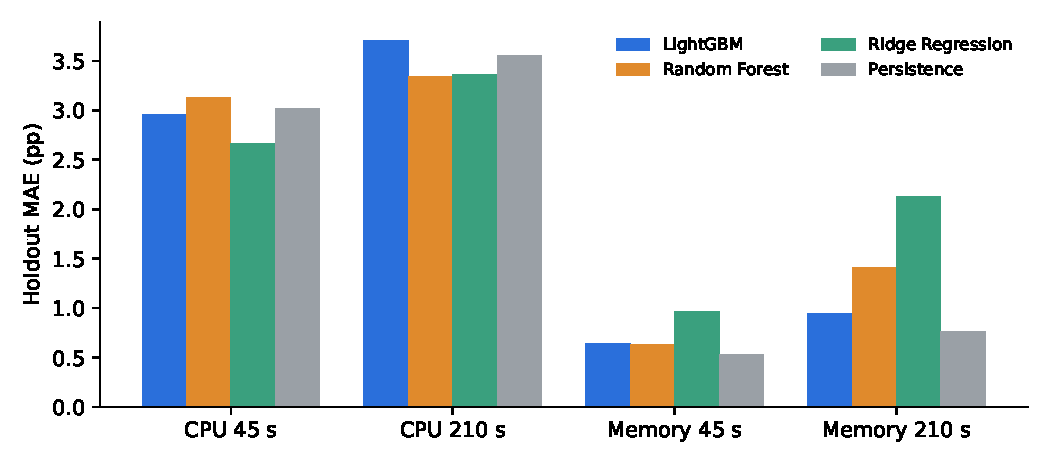
\includegraphics[width=\columnwidth]{figures/holdout_mae.pdf}
\caption{Holdout MAE per target for the three candidates and the persistence
reference.}
\label{fig:mae}
\end{figure}

\begin{figure}[t]
\centering
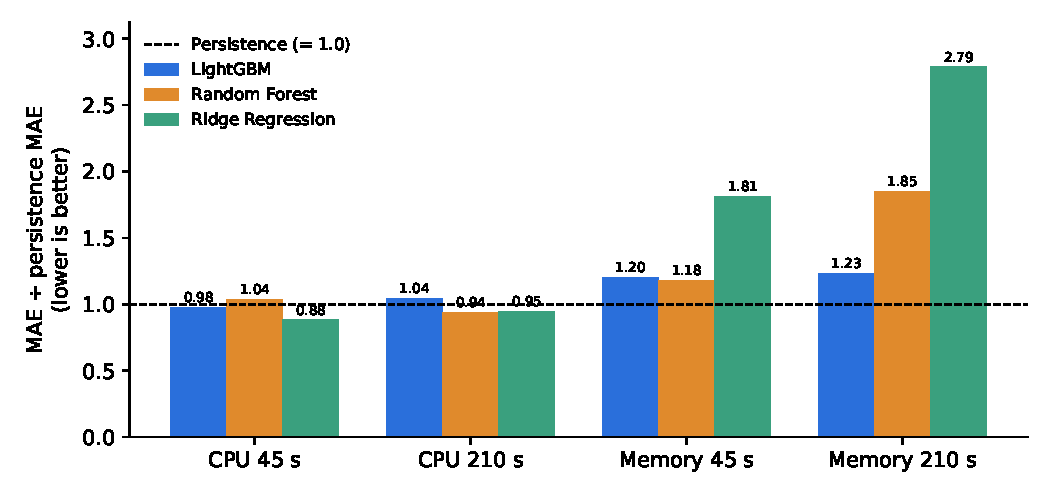
\includegraphics[width=\columnwidth]{figures/relative_error.pdf}
\caption{Each model's holdout MAE divided by persistence's MAE. The dashed
line at 1.0 is ``no change''. Bars above it are worse than persistence and
bars below it are better. LightGBM stays within 1.23 of the line on every
target; Random Forest reaches 1.85 and Ridge 2.79 on memory at 210\,s. Ridge
is below the line on both CPU targets.}
\label{fig:rel}
\end{figure}

Table~\ref{tab:holdout} and Figs.~\ref{fig:mae} and \ref{fig:rel} give the
holdout results. Each candidate is best on at least one target, and the
pattern splits by metric.
\begin{itemize}
  \item \emph{CPU.} Ridge is best at 45\,s (2.66\pp{}, 12\,\% below
        persistence) and close to the best at 210\,s. Random Forest is best at
        210\,s. LightGBM beats persistence at 45\,s by 2\,\% but not at 210\,s.
  \item \emph{Memory.} No model beats persistence. LightGBM is best at
        210\,s and within 0.011\pp{} of the best at 45\,s. Random Forest and
        Ridge degrade badly at 210\,s (85\,\% and 179\,\% worse than
        persistence).
\end{itemize}

\begin{table}[t]
\centering
\caption{Holdout RMSE (pp) and directional accuracy}
\label{tab:rmse}
\footnotesize\setlength{\tabcolsep}{3pt}
\begin{tabular}{@{}l|cccc|cccc@{}}
\toprule
& \multicolumn{4}{c|}{RMSE} & \multicolumn{4}{c}{Directional acc.} \\
Target & LGB & RF & Rdg & Per. & LGB & RF & Rdg & Per. \\
\midrule
CPU 45\,s  & 4.88 & 4.94 & \textbf{4.62} & 5.48 & .54 & .54 & \textbf{.57} & .10 \\
CPU 210\,s & 5.51 & \textbf{5.23} & 5.24 & 6.02 & .54 & \textbf{.56} & .56 & .09 \\
Mem 45\,s  & 1.30 & 1.38 & 1.54 & \textbf{1.13} & .86 & .89 & .81 & \textbf{.92} \\
Mem 210\,s & 1.67 & 3.37 & 2.99 & \textbf{1.37} & .82 & .81 & .41 & \textbf{.85} \\
\bottomrule
\end{tabular}
\end{table}

Table~\ref{tab:rmse} adds a second view. On \emph{RMSE}, which penalises
large errors more heavily, all three models \emph{beat} persistence on both
CPU targets; LightGBM's RMSE is 4.88 versus 5.48 at 45\,s and 5.51 versus
6.02 at 210\,s. The learned models make many small errors on idle samples and
fewer large errors on bursts. Section~\ref{sec:regime} confirms this directly.
Directional accuracy on CPU is about 0.55 for all three models, against 0.10
for persistence. Persistence never predicts a change, so it is scored wrong
whenever CPU moves by more than 2\,\%. On memory, which rarely moves that much,
persistence's directional accuracy is naturally high.

\begin{table}[t]
\centering
\caption{Holdout accuracy in percent, $100 - \mathrm{MAE}$ (the targets are
themselves 0--100\,\%). Persistence scores as well as the models on this
idle-heavy test period.}
\label{tab:accpct}
\begin{tabular}{@{}lcccc@{}}
\toprule
Target & LightGBM & Rand.\ Forest & Ridge & \textit{Persist.} \\
\midrule
CPU, 45\,s   & 97.0 & 96.9 & \textbf{97.3} & \textit{97.0} \\
CPU, 210\,s  & 96.3 & \textbf{96.7} & 96.6 & \textit{96.5} \\
Mem, 45\,s   & 99.4 & \textbf{99.4} & 99.0 & \textit{99.5} \\
Mem, 210\,s  & \textbf{99.1} & 98.6 & 97.9 & \textit{99.2} \\
\midrule
Mean         & \textbf{97.9} & 97.9 & 97.7 & \textit{98.0} \\
\bottomrule
\end{tabular}
\end{table}

For readers who expect a single percentage, Table~\ref{tab:accpct} restates the
holdout MAE as accuracy, $100 - \mathrm{MAE}$, which is one minus the MAE
normalised by the 0--100\,\% range. LightGBM's forecasts are 97.9\,\%
accurate on average: about 97\,\% for CPU and 99\,\% for memory. The measure
is generous on this data, because persistence reaches 98.0\,\% simply by
repeating the current value. It is reported for readability only; the skill
score of Section~\ref{sec:problem}, which compares each model with
persistence directly, remains the basis for model selection.

\subsection{Walk-forward stability}

\begin{table}[t]
\centering
\caption{Walk-forward CV MAE on the training portion, mean $\pm$ s.d.\ over
4 folds.}
\label{tab:cv}
\begin{tabular}{@{}lcccc@{}}
\toprule
Target & LightGBM & Rand.\ Forest & Ridge & \textit{Persist.} \\
\midrule
CPU, 45\,s  & 2.98$\pm$0.89 & \textbf{2.25$\pm$0.43} & 3.28$\pm$1.65 & \textit{2.24$\pm$0.12} \\
CPU, 210\,s & 3.59$\pm$1.28 & \textbf{3.34$\pm$0.96} & 5.65$\pm$4.39 & \textit{2.58$\pm$0.29} \\
Mem, 45\,s  & 1.89$\pm$2.30 & \textbf{1.76$\pm$2.43} & 2.31$\pm$2.39 & \textit{0.69$\pm$0.53} \\
Mem, 210\,s & \textbf{3.28$\pm$4.14} & 3.36$\pm$4.54 & 6.54$\pm$6.74 & \textit{1.14$\pm$1.06} \\
\bottomrule
\end{tabular}
\end{table}

\begin{figure}[t]
\centering
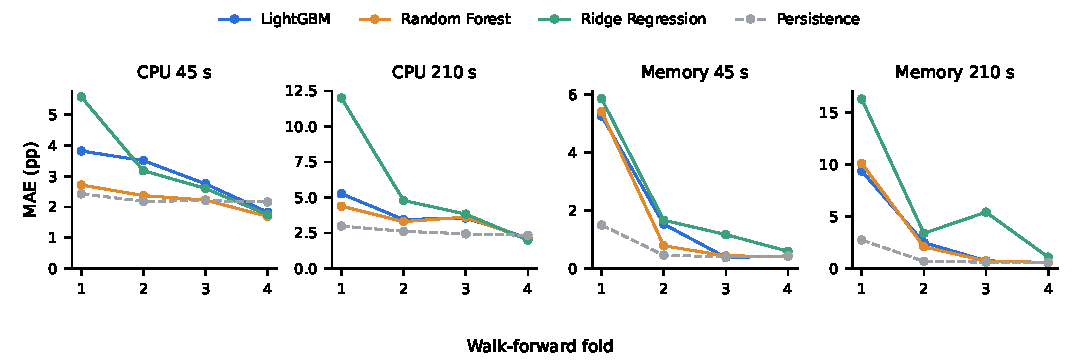
\includegraphics[width=\columnwidth]{figures/cv_folds.pdf}
\caption{Walk-forward MAE per fold. Errors fall sharply as each model sees
more training data (fold~1 trains on the least data), and Ridge is the least
stable.}
\label{fig:folds}
\end{figure}

Table~\ref{tab:cv} and Fig.~\ref{fig:folds} show the cross-validation results.
Here Random Forest has the lowest mean error on three of four targets and
LightGBM on one. Ridge, despite its good CPU holdout, has the widest spread on three of
the four targets, and its fold-1 CPU errors are 1.5--2.7 times those of the
tree models. Every learned model improves steeply from fold~1 to fold~4 as it sees
more data. On memory, the fold-1 errors are several times larger than the later
ones, which is why the standard deviations are so wide. This suggests that the
models are still data-limited.

\subsection{Statistical significance}

\begin{table}[t]
\centering
\caption{Diebold--Mariano tests on absolute error, holdout. $\bar d$ is
LightGBM's mean absolute error minus the rival's, in pp; negative means
LightGBM is better. $^{*}p<0.05$, $^{**}p<0.01$.}
\label{tab:dm}
\footnotesize\setlength{\tabcolsep}{3pt}
\begin{tabular}{@{}l|rr|rr|rr@{}}
\toprule
& \multicolumn{2}{c|}{vs Rand.\ Forest} & \multicolumn{2}{c|}{vs Ridge} & \multicolumn{2}{c}{vs Persist.} \\
Target & $\bar d$ & $p$ & $\bar d$ & $p$ & $\bar d$ & $p$ \\
\midrule
CPU 45\,s  & $-$0.171 & 0.001$^{**}$ & +0.292 & $<$.001$^{**}$ & $-$0.063 & 0.35 \\
CPU 210\,s & +0.363 & $<$.001$^{**}$ & +0.337 & $<$.001$^{**}$ & +0.153 & 0.28 \\
Mem 45\,s  & +0.010 & 0.61 & $-$0.328 & $<$.001$^{**}$ & +0.107 & $<$.001$^{**}$ \\
Mem 210\,s & $-$0.473 & 0.005$^{**}$ & $-$1.189 & $<$.001$^{**}$ & +0.178 & $<$.001$^{**}$ \\
\bottomrule
\end{tabular}
\end{table}

\begin{table*}[t]
\centering
\caption{Holdout skill $S$ with 95\,\% moving-block bootstrap intervals}
\label{tab:ci}
\begin{tabular}{@{}lccc@{}}
\toprule
Target & LightGBM & Random Forest & Ridge \\
\midrule
CPU 45\,s  & \phantom{$-$}0.02 [$-$0.04, 0.10] & $-$0.04 [$-$0.14, 0.05] & \phantom{$-$}\textbf{0.12 [0.07, 0.18]} \\
CPU 210\,s & $-$0.04 [$-$0.15, 0.05] & \phantom{$-$}0.06 [$-$0.00, 0.12] & \phantom{$-$}0.05 [$-$0.03, 0.12] \\
Mem 45\,s  & $-$0.20 [$-$0.29, $-$0.11] & $-$0.18 [$-$0.33, $-$0.04] & $-$0.81 [$-$0.98, $-$0.62] \\
Mem 210\,s & $-$0.23 [$-$0.33, $-$0.12] & $-$0.85 [$-$1.41, $-$0.38] & $-$1.79 [$-$2.31, $-$1.28] \\
\bottomrule
\end{tabular}
\end{table*}

Tables~\ref{tab:dm} and \ref{tab:ci} test how reliable the differences are.
\begin{itemize}
  \item \emph{LightGBM vs Random Forest.} LightGBM is significantly better on
        CPU 45\,s ($p=0.001$) and memory 210\,s ($p=0.005$). Random Forest is
        significantly better on CPU 210\,s ($p<0.001$). There is no
        significant difference on memory 45\,s ($p=0.61$). The head-to-head
        record is two wins, one loss and one tie, the same as without
        preprocessing.
  \item \emph{LightGBM vs Ridge.} The record splits cleanly by metric. Ridge
        is significantly better on both CPU targets and LightGBM on both
        memory targets (all $p<0.001$). LightGBM's memory advantage (0.33 and
        1.19\pp) is larger than Ridge's CPU advantage (0.29 and 0.34\pp).
  \item \emph{LightGBM vs persistence.} On CPU, LightGBM is statistically
        indistinguishable from persistence ($p=0.35$ and $0.28$), and both of
        its skill intervals contain zero. On memory it is significantly worse.
\end{itemize}
Only one model--target pair has a skill interval entirely above zero: Ridge on
CPU 45\,s, at $[0.07,0.18]$. It is the only place in this study where a
learned model beats persistence reliably, and it appears only after
preprocessing.

\subsection{Effect of preprocessing}\label{sec:prepeffect}

\begin{figure}[t]
\centering
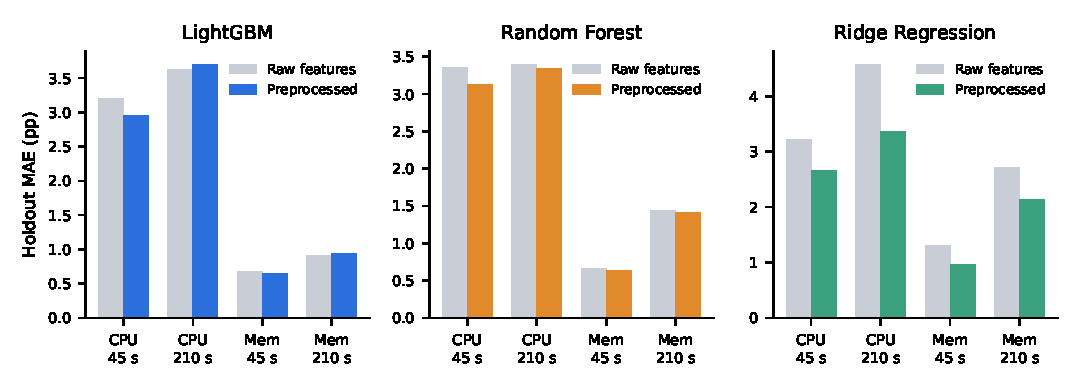
\includegraphics[width=\columnwidth]{figures/preprocessing_effect.pdf}
\caption{Holdout MAE per model with raw features (grey) and after
preprocessing (colour). Ridge improves on every target; the tree models
change little.}
\label{fig:prepeffect}
\end{figure}

\begin{table}[t]
\centering
\caption{Holdout skill $S$ with raw features $\to$ after preprocessing}
\label{tab:prepeffect}
\footnotesize\setlength{\tabcolsep}{3pt}
\begin{tabular}{@{}lccc@{}}
\toprule
Target & LightGBM & Random Forest & Ridge \\
\midrule
CPU 45\,s  & $-$0.05 $\to$ +0.02 & $-$0.10 $\to$ $-$0.04 & $-$0.05 $\to$ \textbf{+0.12} \\
CPU 210\,s & \phantom{+}0.00 $\to$ $-$0.04 & +0.06 $\to$ +0.06 & $-$0.26 $\to$ \textbf{+0.05} \\
Mem 45\,s  & $-$0.18 $\to$ $-$0.20 & $-$0.17 $\to$ $-$0.18 & $-$1.29 $\to$ $-$0.81 \\
Mem 210\,s & $-$0.13 $\to$ $-$0.23 & $-$0.78 $\to$ $-$0.85 & $-$2.33 $\to$ $-$1.79 \\
\midrule
Mean       & $-$0.090 $\to$ $-$0.113 & $-$0.245 $\to$ $-$0.252 & $-$0.984 $\to$ $-$0.607 \\
\bottomrule
\end{tabular}
\end{table}

We ran the whole comparison twice, with and without preprocessing
(Fig.~\ref{fig:prepeffect}, Table~\ref{tab:prepeffect}). We compare skill
rather than raw MAE, because removing warm-up rows also changes the test set,
and skill measures each model against persistence on the same rows. The effect
depends strongly on the model family.
\begin{itemize}
  \item \emph{Ridge gains the most}: its mean skill rises from $-0.98$ to
        $-0.61$, and both CPU targets turn positive. A linear model is
        sensitive to exactly the problems preprocessing fixes. Byte rates
        spanning six orders of magnitude dominate an unscaled linear fit, and
        29 near-duplicate columns make its coefficients unstable. The log
        transform and redundancy filter remove both problems.
  \item \emph{The tree models change little} (mean skill $-0.090\to-0.113$
        for LightGBM, $-0.245\to-0.252$ for Random Forest). This is expected.
        A tree splits on thresholds, so a monotone transform such as the log
        leaves its possible splits unchanged, and trees tolerate redundant
        columns. The small shifts come from the warm-up rows and the dropped
        columns changing which splits are chosen. LightGBM gains on CPU 45\,s
        and loses on memory 210\,s.
\end{itemize}
Preprocessing is therefore not a free win for every model, but it is what
makes a fair comparison possible. Without it, Ridge was being judged on inputs
it cannot use.

\subsection{Where the models win and lose (RQ2)}\label{sec:regime}

\begin{figure}[t]
\centering
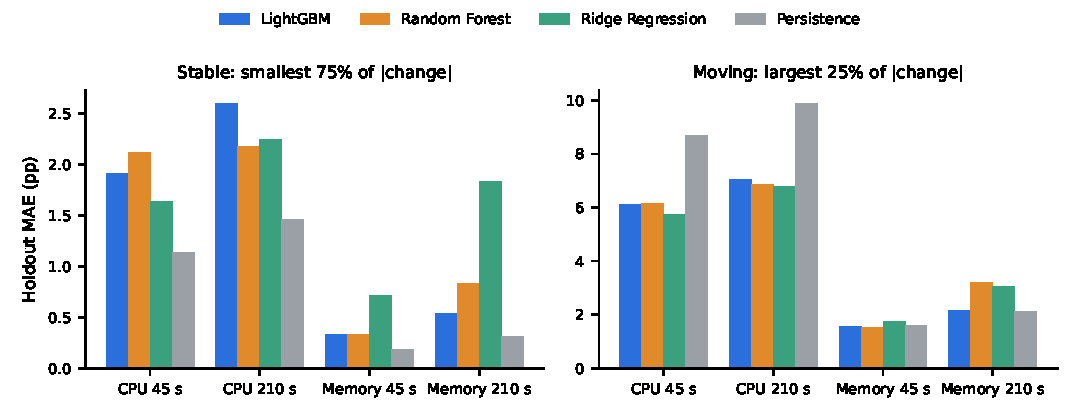
\includegraphics[width=\columnwidth]{figures/regimes.pdf}
\caption{Holdout MAE split by regime. Left: the 75\,\% of samples with the
smallest actual change, where persistence is near-perfect. Right: the 25\,\%
with the largest change, where every learned model cuts CPU error by about
30\,\% against persistence.}
\label{fig:regimes}
\end{figure}

Fig.~\ref{fig:regimes} answers RQ2. The negative average skill hides two very
different situations.
\begin{itemize}
  \item \textbf{Moving regime} (largest 25\,\% of changes). On CPU,
        LightGBM's MAE is 6.10\pp{} against persistence's 8.67\pp{} at 45\,s
        (30\,\% lower) and 7.05\pp{} against 9.87\pp{} at 210\,s (29\,\%
        lower). Ridge does slightly better (5.74 and 6.77, 34\,\% and
        31\,\% lower) and Random Forest is similar (6.15 and 6.84). On
        memory, LightGBM ties with persistence (1.57 vs 1.58 at 45\,s, and
        2.18 vs 2.13 at 210\,s), while Random Forest and Ridge are clearly
        worse at 210\,s.
  \item \textbf{Stable regime} (smallest 75\,\%). Here persistence is
        excellent (1.13\pp{} on CPU at 45\,s) and every model is worse
        (LightGBM 1.91, Ridge 1.64). The models occasionally predict a small
        change that does not happen, and that costs a little error on each of
        the many stable samples.
\end{itemize}
Because three quarters of the samples are stable, their small losses outweigh
the large gains on the moving samples. This happens on MAE in particular,
which weights every sample equally. It also explains why the learned models
win on RMSE (Table~\ref{tab:rmse}) but mostly lose on MAE. The learned models
\emph{have} learned something real about how CPU load changes. What they
cannot yet do is recognise, before the fact, that the machine is in a stable
period and stay quiet.

\subsection{What the model relies on (RQ3)}

\begin{figure}[t]
\centering
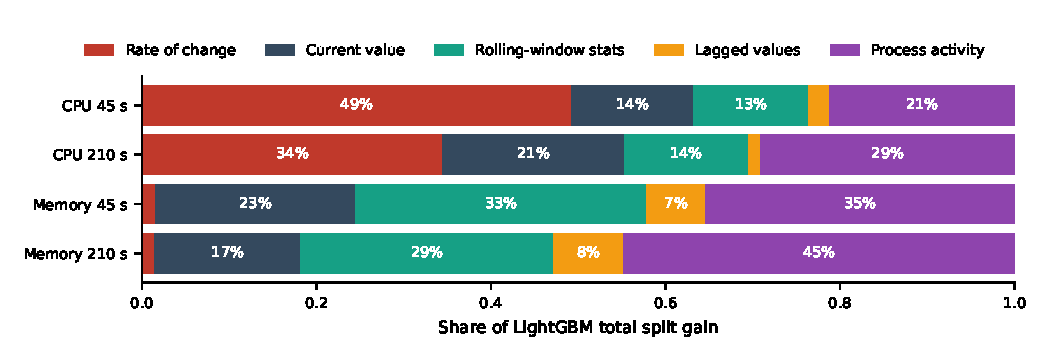
\includegraphics[width=\columnwidth]{figures/importance.pdf}
\caption{Share of LightGBM's total split gain by feature group, per target.}
\label{fig:importance}
\end{figure}

Fig.~\ref{fig:importance} shows LightGBM's split-gain importance by feature
group. For CPU, the single most important feature is the CPU rate of change:
49\,\% of total gain at 45\,s and 34\,\% at 210\,s. The current value comes
next (14\,\% and 21\,\%). This fits the regime result, since the model mostly
learns how the current trend continues. For memory, rolling-window statistics
(29--33\,\%) and process-activity features (35--45\,\%) matter more. The
largest single process features for memory at 210\,s are the recent CPU use of
newly started processes, the minimum thread count and a process-launch burst
indicator. Process features make up 65\,\% of the kept columns (145 of 224)
and receive 21--45\,\% of the gain, so each one is individually less important
than a typical system feature. Gain importance shows what the model
\emph{uses}, not that a feature \emph{improves} accuracy. We therefore do not
claim that process features improve accuracy on this data.

\subsection{Cost}

\begin{figure}[t]
\centering
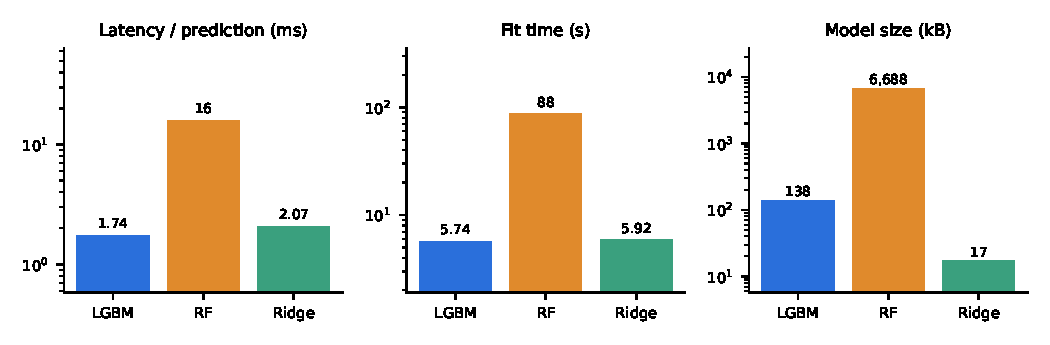
\includegraphics[width=\columnwidth]{figures/cost.pdf}
\caption{Cost per model, averaged over the four targets (log scale). Latency
and fit time include the preprocessing step.}
\label{fig:cost}
\end{figure}

Fig.~\ref{fig:cost} compares cost. Including preprocessing, LightGBM predicts
one row in 1.74\,ms, against 2.07\,ms for Ridge and 15.8\,ms for Random Forest
($9\times$ slower). The preprocessing transform itself adds about 1.4\,ms per
row for every model. The raw-feature run measured the models alone at
0.33\,ms (LightGBM), 0.69\,ms (Ridge) and 14.1\,ms (Random Forest).
LightGBM and Ridge fit in about 6\,s, of which about 4.5\,s is the correlation
scan of the preprocessing step, while Random Forest takes 82--97\,s. LightGBM
models are about 138\,kB, Random Forest models 4.5--10.0\,MB and Ridge models
17\,kB. PRISM runs four forecasters every 5\,s within a 3\,\% CPU budget and
retrains on the user's own machine, so these differences matter in practice.

\subsection{Choice and reasoning}

\begin{table}[t]
\centering
\caption{Summary used for selection (preprocessed data)}
\label{tab:summary}
\footnotesize\setlength{\tabcolsep}{3pt}
\begin{tabular}{@{}lccc@{}}
\toprule
 & LightGBM & Rand.\ Forest & Ridge \\
\midrule
Mean holdout skill $S$           & \textbf{$-$0.113} & $-$0.252 & $-$0.607 \\
Worst target vs.\ persistence    & \textbf{+23\,\%} & +85\,\% & +179\,\% \\
Best of 3, holdout targets       & 1/4 & 2/4 & 1/4 \\
Best of 3, CV targets            & 1/4 & \textbf{3/4} & 0/4 \\
Beats persistence reliably       & -- & -- & CPU 45\,s \\
LightGBM's DM record vs.\ rival  & -- & 2W 1L 1T & 2W 2L \\
Latency per prediction           & \textbf{1.74\,ms} & 15.8\,ms & 2.07\,ms \\
Fit time per target              & $\approx$6\,s & $\approx$88\,s & $\approx$6\,s \\
Model size                       & 138\,kB & 4.5--10\,MB & \textbf{17\,kB} \\
\bottomrule
\end{tabular}
\end{table}

Under the rule fixed in advance, \textbf{LightGBM is selected}
(Table~\ref{tab:summary}). Its mean skill is 0.139 above Random Forest's and
0.494 above Ridge's, far outside the 0.02 tie-break band. The choice is the
same as without preprocessing, but the evidence is now more mixed, and we
report it as such. Ridge is the best CPU model, and Random Forest has the
better cross-validation record. Four arguments support LightGBM as the
single model PRISM ships.
\begin{enumerate}
  \item \emph{It has no bad target.} LightGBM is at most 23\,\% worse than
        persistence on any target. Random Forest is 85\,\% worse and Ridge
        179\,\% worse on memory at 210\,s, which is the horizon a user most
        needs for planning. A monitor that is occasionally very wrong damages
        trust more than one that is consistently close.
  \item \emph{Its wins are large and its losses small.} Against Random
        Forest it wins two targets significantly and loses one. Against Ridge
        its memory wins (0.33 and 1.19\pp) outweigh its CPU losses (0.29 and
        0.34\pp).
  \item \emph{Cost.} It has the lowest latency and a fit time about
        $15\times$ shorter than Random Forest's, which makes frequent
        on-device retraining practical.
  \item \emph{Fit with the rest of the system.} It handles the missing lag
        features that follow collector gaps natively, supports exact TreeSHAP
        for the diagnosis module, and produces small models that are cheap to
        version and roll back.
\end{enumerate}
The results also suggest a better design than any single model: Ridge for CPU
and LightGBM for memory. We do not adopt it here. Choosing a model per target
after seeing the test results would break the rule we fixed in advance, so it
has to be confirmed on new data first (Section~\ref{sec:discussion}).

\subsection{Comparison with statistical baselines and the gate}

\begin{table}[t]
\centering
\caption{Walk-forward MAE of LightGBM versus the statistical baselines
(earlier evaluation run on raw features, same data window, 113{,}882 samples).}
\label{tab:baselines}
\begin{tabular}{@{}lcccc@{}}
\toprule
Target & LightGBM & Persist. & Mov.\ avg. & Holt ETS \\
\midrule
CPU, 45\,s  & 3.15 & 2.13 & \textbf{1.81} & 2.87 \\
CPU, 210\,s & 3.34 & 2.50 & \textbf{2.19} & 7.55 \\
Mem, 45\,s  & 2.85 & 1.07 & \textbf{1.01} & 1.66 \\
Mem, 210\,s & 3.19 & 1.75 & \textbf{1.68} & 4.90 \\
\bottomrule
\end{tabular}
\end{table}

Table~\ref{tab:baselines} shows the separate harness that feeds the deployment
gate. The moving average has the lowest error on all four targets, so the gate
(Section~\ref{sec:gate}) currently serves the moving average, not LightGBM.
This agrees with everything above: on idle-dominated data, a model that
smooths the recent past is hard to beat on average error. Fig.~\ref{fig:pva}
shows the cost of that choice in the live system. The served forecast follows
a sharp memory rise only after a delay, which is exactly the moving-regime
weakness that the learned models address.

\begin{figure}[t]
\centering
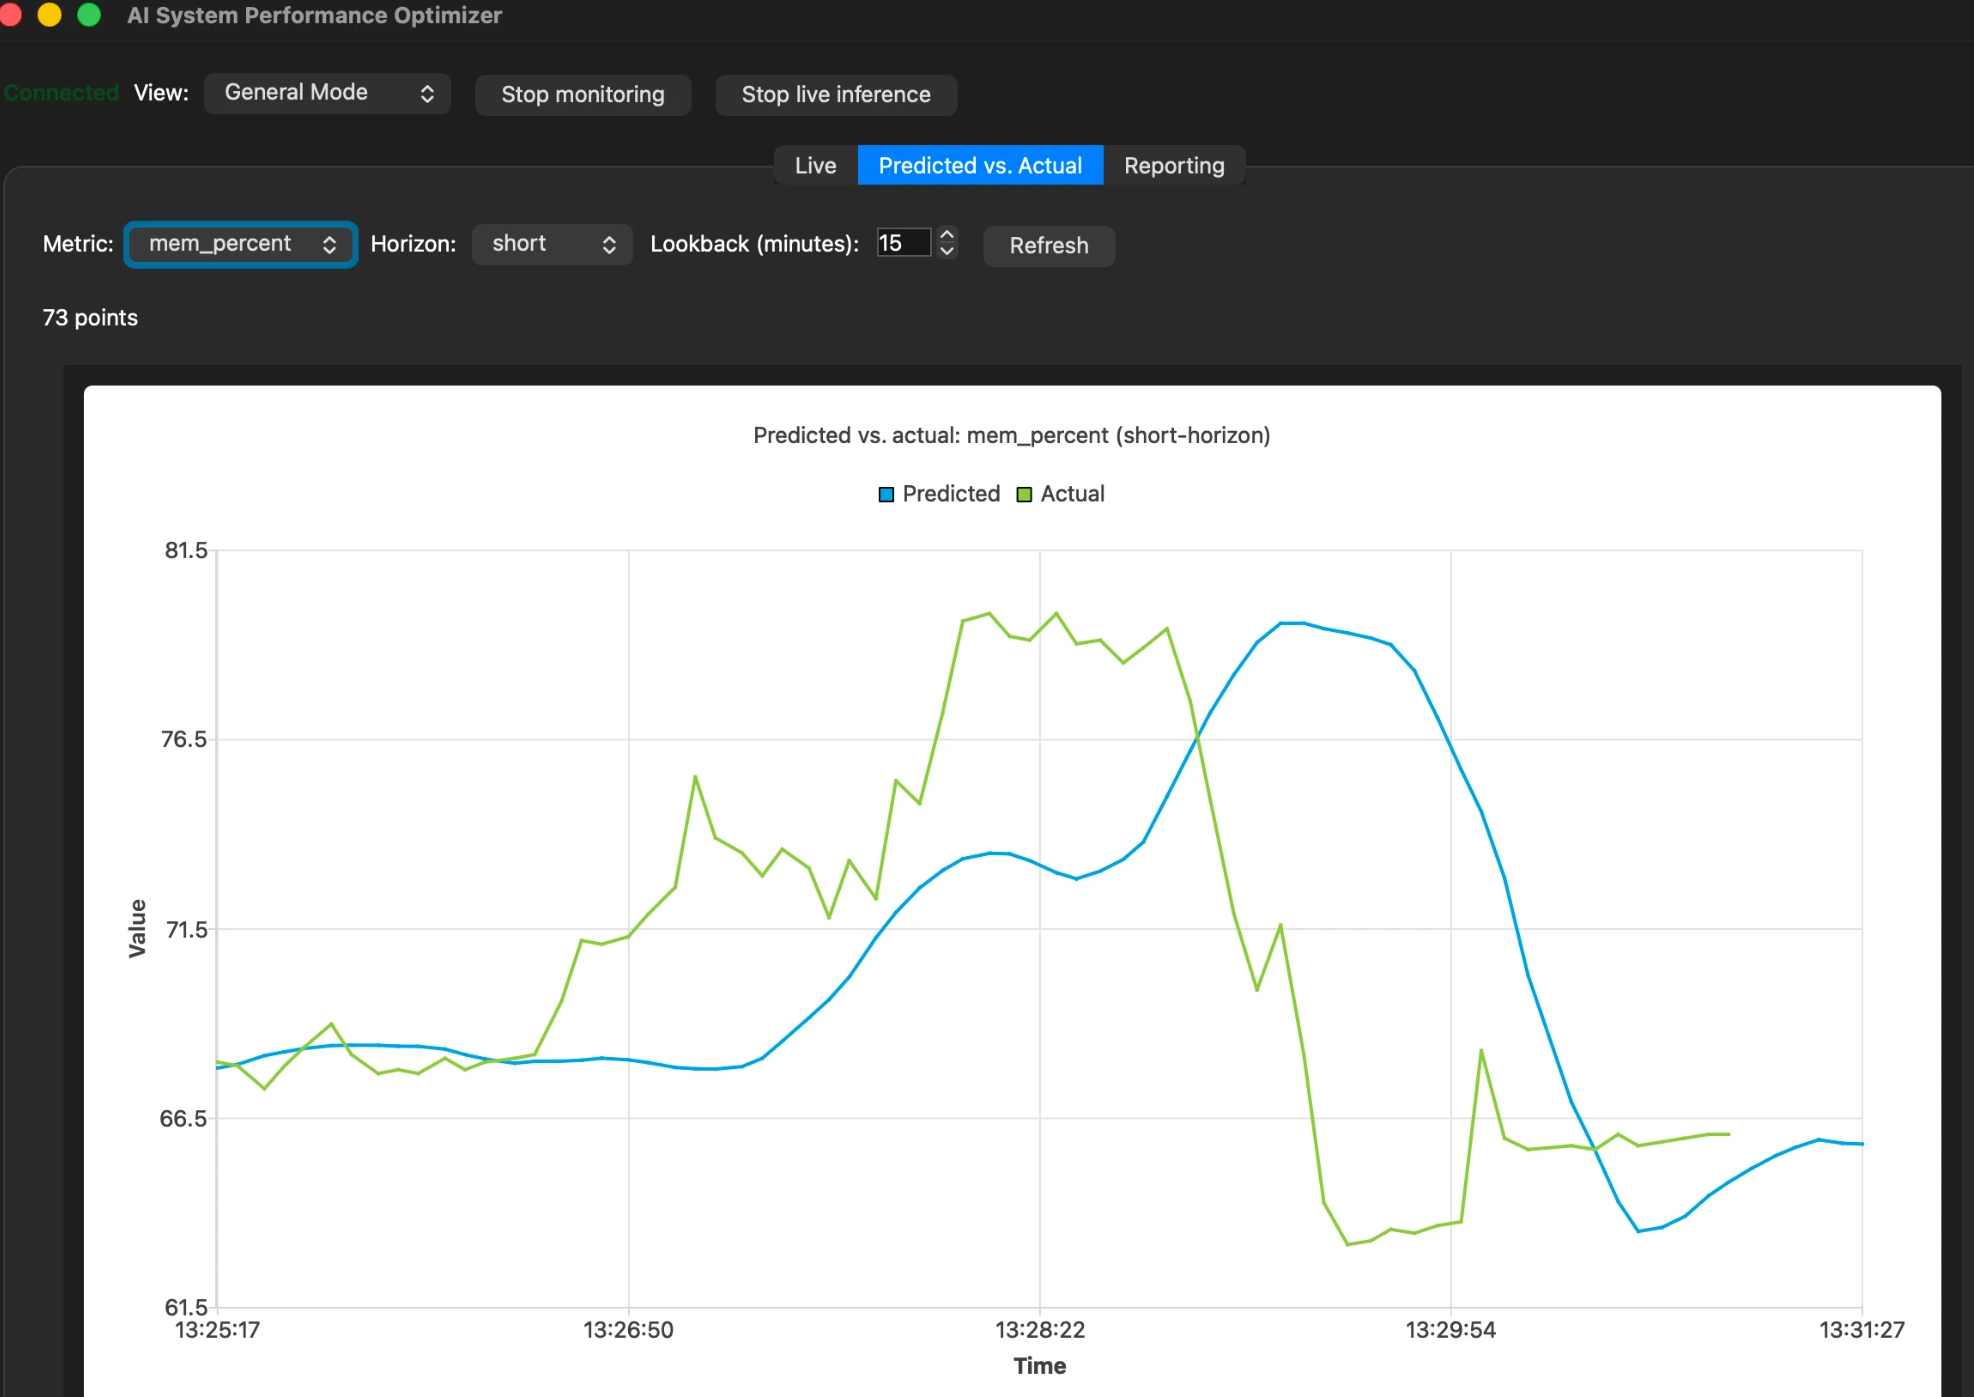
\includegraphics[width=\columnwidth]{figures/predicted_vs_actual.png}
\caption{Predicted-vs-Actual tab (memory, short horizon). The served,
gate-selected baseline forecast (blue) lags a sharp rise and fall in actual
memory use (green) by roughly the forecast horizon.}
\label{fig:pva}
\end{figure}

\subsection{Contention classifier and overhead}
The contention label is rare. In a 113{,}882-sample window, 1.5\,\% of samples
are positive, and all of them fall in the training portion, so the
chronological holdout contains \emph{no} positives. Holdout precision, recall
and F1 are therefore undefined, and we report them as undefined rather than as
a score. A classifier trained on a genuine recorded pressure event (swap up to
91.8\,\%, CPU up to 78.7\,\%) is deployed and drives the live contention strip
in Fig.~\ref{fig:dashboard}. Its accuracy will be measured once a second,
independent event falls inside a holdout window. Overheads are within budget:
2.26\,\% CPU and 3.48\,MB/h of database growth.

%=====================================================================
\section{Discussion}\label{sec:discussion}
%=====================================================================

\subsection{Why persistence is so hard to beat}
Persistence is close to the best possible predictor whenever a series changes
slowly relative to the forecast horizon. On this machine, CPU is below 20\,\%
in 96.7\,\% of samples, and 80\,\% of memory samples lie within a 17.5-point
band. Over 45\,s, the typical change is smaller than the noise. A learned model
has to pay for its ability to predict change: it sometimes predicts a change
that does not happen. The regime analysis shows that this price is small per
sample but applies to the majority of samples. Negative average skill on this
data therefore reflects the workload, not a bug. The same effect is well known
in forecasting generally, where naive benchmarks are routinely hard to
beat~\cite{hyndman2021fpp}.

\subsection{What preprocessing taught us}
Preprocessing changed which model is best on CPU at 45\,s, from a near-tie
between LightGBM and Ridge (3.21 vs 3.21\pp) to a clear, statistically
reliable Ridge win. It did not
change the winner, because the tree models are largely insensitive to it.
Two lessons follow. First, a model comparison is only fair when each model gets
inputs it can use; comparing a linear model on raw, skewed, redundant features
understated it badly. Second, the fitted steps must be refitted inside every
cross-validation fold. Fitting them once on all the data would let the choice
of columns see the test period.

\subsection{Implications for design}
The results point to two next steps. The first is a \emph{per-target}
forecaster (Ridge for CPU, LightGBM for memory), to be confirmed on new data.
The second is a \emph{regime-aware} forecaster. A lightweight gate would
predict whether the next window will be stable, using the rate-of-change and
rolling-variance features that already dominate LightGBM's importance. It
would serve persistence in stable periods and a learned model during
transitions. Recovering even part of the moving-regime gain (about 30\,\% on
CPU) without the stable-regime loss would give positive skill and let the
deployment gate promote an ML model on its own evidence. The MAE-versus-RMSE
split also suggests that the metric should follow the product goal: a monitor
exists to catch bursts, which is closer to what RMSE rewards.

\subsection{Threats to validity}
\begin{enumerate}
  \item \emph{One machine, one user, two days of recorded data.} The results
        may not generalise to other workloads, and the fold-to-fold trend in
        Fig.~\ref{fig:folds} suggests that the models are still data-limited.
  \item \emph{No tuning.} LightGBM uses production defaults and the others
        use common defaults. Tuning could change the ordering.
  \item \emph{Preprocessing is not yet in the live app.} It is used in the
        comparison experiments and is a tested module, but the deployed
        forecaster does not call it yet.
  \item \emph{The raw and preprocessed runs use slightly different test
        rows}, because warm-up rows are removed. We compare them by skill,
        which is measured against persistence on the same rows.
  \item \emph{Different snapshot for Table~\ref{tab:baselines}.} It comes
        from an earlier run on raw features with its own training code, so
        only the ranking within it is comparable with the other tables.
  \item \emph{The regime split conditions on the outcome}, and \emph{gain
        importance is not causality}. Both explain the results; neither is a
        deployable rule.
\end{enumerate}

%=====================================================================
\section{Conclusion and Future Work}
%=====================================================================
PRISM is a complete, tested, low-overhead pipeline for predictive and
explainable desktop monitoring. We added a preprocessing stage that removes
warm-up rows after gaps, log-transforms skewed byte rates and drops constant
and redundant features. All learned steps are fitted on training data only.
With it, we compared three ML forecasters under a selection rule fixed in
advance. LightGBM had the best mean skill and the smallest worst case, won its
head-to-head against Random Forest, and was the cheapest to run. It is
therefore PRISM's forecasting model. Preprocessing turned Ridge into the best
CPU forecaster, the only model that reliably beat persistence anywhere. We have
also stated clearly what the data does not yet show: on idle-dominated usage,
no learned forecaster beats persistence on average, and the deployment gate
correctly keeps a moving-average baseline in service. The regime analysis
shows why, and it shows that the learned models add value exactly where a
monitor needs it, when load is changing.

Future work, in order of expected impact:
\begin{enumerate}
  \item a regime-aware or per-target forecaster (persistence when stable,
        Ridge for CPU, LightGBM for memory), confirmed on new data;
  \item building the preprocessing stage into the live app and the deployed
        models;
  \item longer and more varied collection across several machines and users,
        so that contention events fall in the holdout and the classifier can
        be graded;
  \item hyperparameter tuning of all candidates under the same protocol;
  \item calibrated prediction intervals, and verification on Windows.
\end{enumerate}

\section*{Reproducibility}
{\raggedright
\begin{itemize}
  \item Three-model comparison: \texttt{python scripts/compare\_models.py}
        (\texttt{--raw} for the unprocessed run).
  \item Significance, bootstrap, regime and importance analysis:
        \texttt{python scripts/paper\_analysis.py} (on the frozen snapshot;
        reproduces every holdout MAE in Table~\ref{tab:holdout} exactly).
  \item Figures: \texttt{python scripts/paper\_figures.py}.
  \item Preprocessing module and tests:
        \texttt{features/preprocessing.py},
        \texttt{tests/test\_features\_preprocessing.py}.
  \item Statistical-baseline table: \texttt{aiperfopt evaluate --report}.
\end{itemize}
}

\begin{thebibliography}{00}
\bibitem{gong2010press} Z.~Gong, X.~Gu, and J.~Wilkes, ``PRESS: PRedictive
Elastic reSource Scaling for cloud systems,'' in \emph{Proc.\ Int.\ Conf.\
Network and Service Management (CNSM)}, 2010, pp.~9--16.
\bibitem{roy2011autoscaling} N.~Roy, A.~Dubey, and A.~Gokhale, ``Efficient
autoscaling in the cloud using predictive models for workload forecasting,'' in
\emph{Proc.\ IEEE Int.\ Conf.\ Cloud Computing (CLOUD)}, 2011, pp.~500--507.
\bibitem{calheiros2015arima} R.~N.~Calheiros, E.~Masoumi, R.~Ranjan, and
R.~Buyya, ``Workload prediction using ARIMA model and its impact on cloud
applications' QoS,'' \emph{IEEE Trans.\ Cloud Computing}, vol.~3, no.~4,
pp.~449--458, 2015.
\bibitem{friedman2001gbm} J.~H.~Friedman, ``Greedy function approximation: A
gradient boosting machine,'' \emph{Annals of Statistics}, vol.~29, no.~5,
pp.~1189--1232, 2001.
\bibitem{chen2016xgboost} T.~Chen and C.~Guestrin, ``XGBoost: A scalable tree
boosting system,'' in \emph{Proc.\ ACM SIGKDD Int.\ Conf.\ Knowledge Discovery
and Data Mining}, 2016, pp.~785--794.
\bibitem{ke2017lightgbm} G.~Ke \emph{et al.}, ``LightGBM: A highly efficient
gradient boosting decision tree,'' in \emph{Advances in Neural Information
Processing Systems (NeurIPS)}, vol.~30, 2017.
\bibitem{breiman2001rf} L.~Breiman, ``Random forests,'' \emph{Machine
Learning}, vol.~45, no.~1, pp.~5--32, 2001.
\bibitem{hoerl1970ridge} A.~E.~Hoerl and R.~W.~Kennard, ``Ridge regression:
Biased estimation for nonorthogonal problems,'' \emph{Technometrics}, vol.~12,
no.~1, pp.~55--67, 1970.
\bibitem{grinsztajn2022tree} L.~Grinsztajn, E.~Oyallon, and G.~Varoquaux,
``Why do tree-based models still outperform deep learning on typical tabular
data?'' in \emph{Advances in Neural Information Processing Systems (NeurIPS),
Datasets and Benchmarks Track}, 2022.
\bibitem{chandola2009anomaly} V.~Chandola, A.~Banerjee, and V.~Kumar,
``Anomaly detection: A survey,'' \emph{ACM Computing Surveys}, vol.~41, no.~3,
pp.~1--58, 2009.
\bibitem{liu2008iforest} F.~T.~Liu, K.~M.~Ting, and Z.-H.~Zhou, ``Isolation
forest,'' in \emph{Proc.\ IEEE Int.\ Conf.\ Data Mining (ICDM)}, 2008,
pp.~413--422.
\bibitem{lundberg2017shap} S.~M.~Lundberg and S.-I.~Lee, ``A unified approach
to interpreting model predictions,'' in \emph{Advances in Neural Information
Processing Systems (NeurIPS)}, vol.~30, 2017.
\bibitem{lundberg2020treeshap} S.~M.~Lundberg \emph{et al.}, ``From local
explanations to global understanding with explainable AI for trees,''
\emph{Nature Machine Intelligence}, vol.~2, no.~1, pp.~56--67, 2020.
\bibitem{tashman2000} L.~J.~Tashman, ``Out-of-sample tests of forecasting
accuracy: An analysis and review,'' \emph{Int.\ J.\ Forecasting}, vol.~16,
no.~4, pp.~437--450, 2000.
\bibitem{bergmeir2012} C.~Bergmeir and J.~M.~Ben\'itez, ``On the use of
cross-validation for time series predictor evaluation,'' \emph{Information
Sciences}, vol.~191, pp.~192--213, 2012.
\bibitem{hyndman2006accuracy} R.~J.~Hyndman and A.~B.~Koehler, ``Another look
at measures of forecast accuracy,'' \emph{Int.\ J.\ Forecasting}, vol.~22,
no.~4, pp.~679--688, 2006.
\bibitem{hyndman2021fpp} R.~J.~Hyndman and G.~Athanasopoulos,
\emph{Forecasting: Principles and Practice}, 3rd~ed.\ Melbourne, Australia:
OTexts, 2021.
\bibitem{diebold1995dm} F.~X.~Diebold and R.~S.~Mariano, ``Comparing
predictive accuracy,'' \emph{J.\ Business \& Economic Statistics}, vol.~13,
no.~3, pp.~253--263, 1995.
\bibitem{newey1987hac} W.~K.~Newey and K.~D.~West, ``A simple, positive
semi-definite, heteroskedasticity and autocorrelation consistent covariance
matrix,'' \emph{Econometrica}, vol.~55, no.~3, pp.~703--708, 1987.
\bibitem{kunsch1989block} H.~R.~K\"unsch, ``The jackknife and the bootstrap
for general stationary observations,'' \emph{Annals of Statistics}, vol.~17,
no.~3, pp.~1217--1241, 1989.
\bibitem{pedregosa2011sklearn} F.~Pedregosa \emph{et al.}, ``Scikit-learn:
Machine learning in Python,'' \emph{J.\ Machine Learning Research}, vol.~12,
pp.~2825--2830, 2011.
\end{thebibliography}

\end{document}
